
\subsection{Méthodologie}
\DylanSpeak
\begin{frame}{Résultats méthodologiques}
	\begin{itemize}
	\item Réalisation des issues \scriptsize{(- de 10\% d’issues encore ouvertes)}
	\normalsize
	\item Principales fonctionnalités implémentés
	\item Mise en place de Scrum \scriptsize{(revues et rétrospectives)}
	\end{itemize}
	\begin{figure}[H]
		\centering
		\includegraphics[width=0.8\linewidth]{"images/Results/methodo/badges"}
		\caption{\textit{Badges} du projet BandStorm}
		\label{fig:badges}
	\end{figure}\end{frame}
\SteveSpeak
\begin{frame}{Mise en place de SonarQube}
\begin{figure}
	\centering
	\includegraphics[width=0.95\linewidth]{"images/Results/methodo/sonar"}
	\caption{Tableau de bord de SonarQube}
	\label{fig:sonar}
\end{figure}
	
\end{frame}

\begin{frame}{Mise en place de Scrum}
	
\begin{figure}
\centering
\includegraphics[width=0.95\linewidth]{"images/Results/methodo/burndown"}
\caption{\textit{Burn-down chart} du Sprint 1}
\label{fig:burndown}
\end{figure}

\end{frame}

\ZacSpeak
\subsection{Produit}
\begin{frame}
\only<1>{
\begin{figure}
\centering
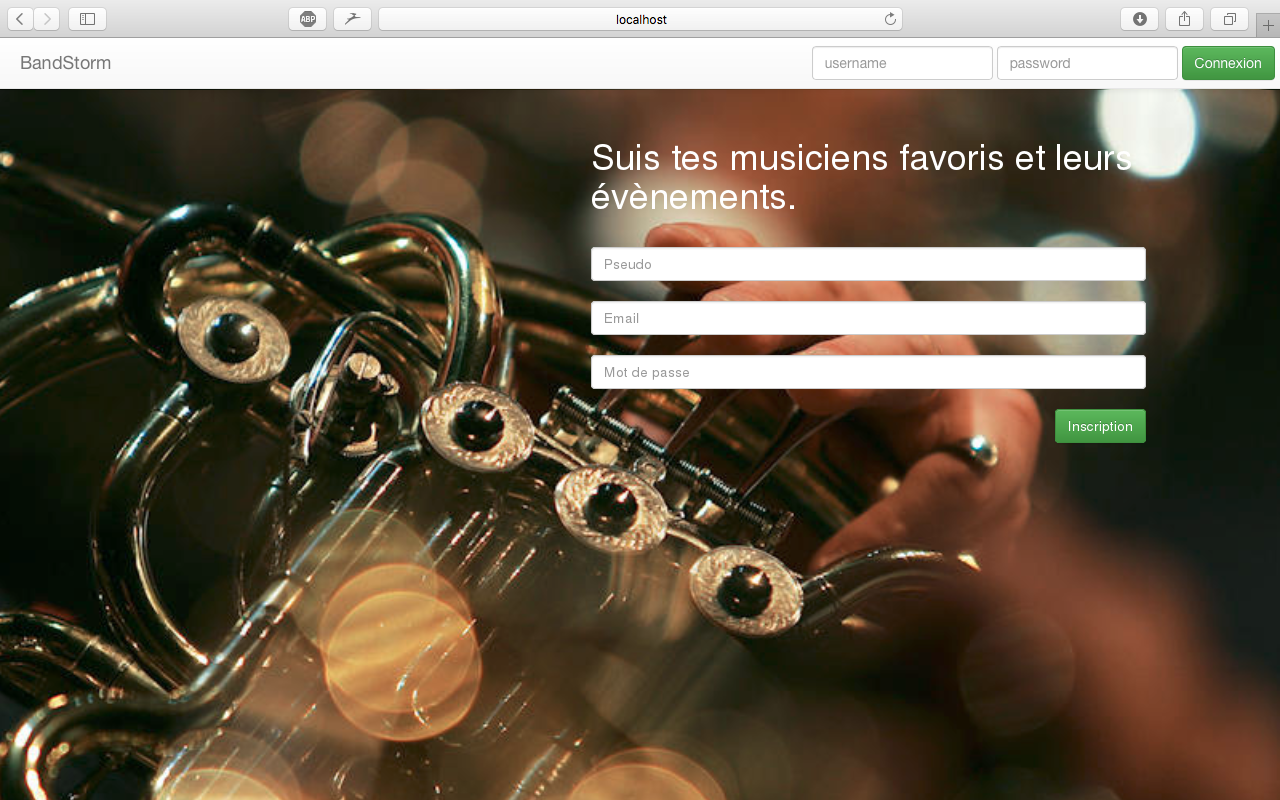
\includegraphics[width=0.95\linewidth]{images/Results/product/scshot1}
\caption{Page d'accueil des visiteurs}
\label{fig:scshot1}
\end{figure}
}
\only<2>{
\begin{figure}
\centering
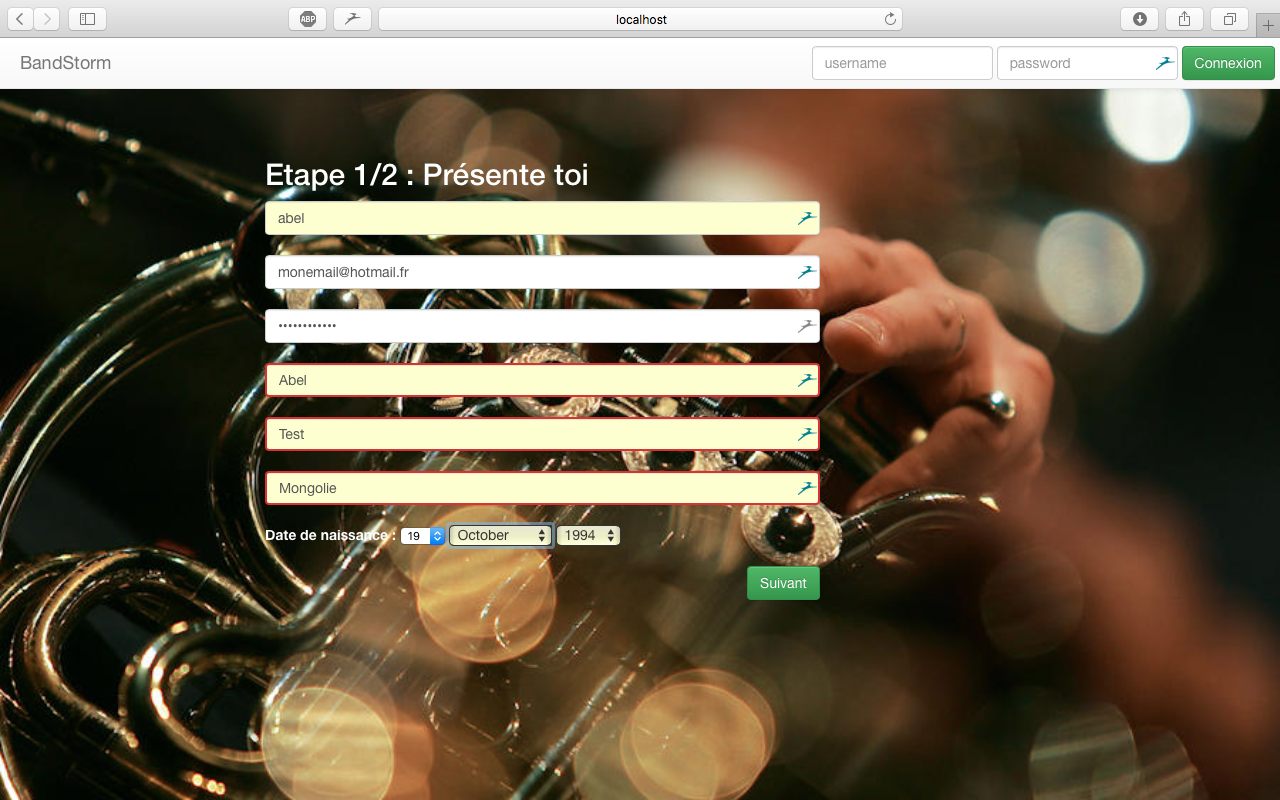
\includegraphics[width=0.95\linewidth]{images/Results/product/scshot2}
\caption{Inscription}
\label{fig:scshot2}
\end{figure}
}

\only<3>{
\begin{figure}
\centering
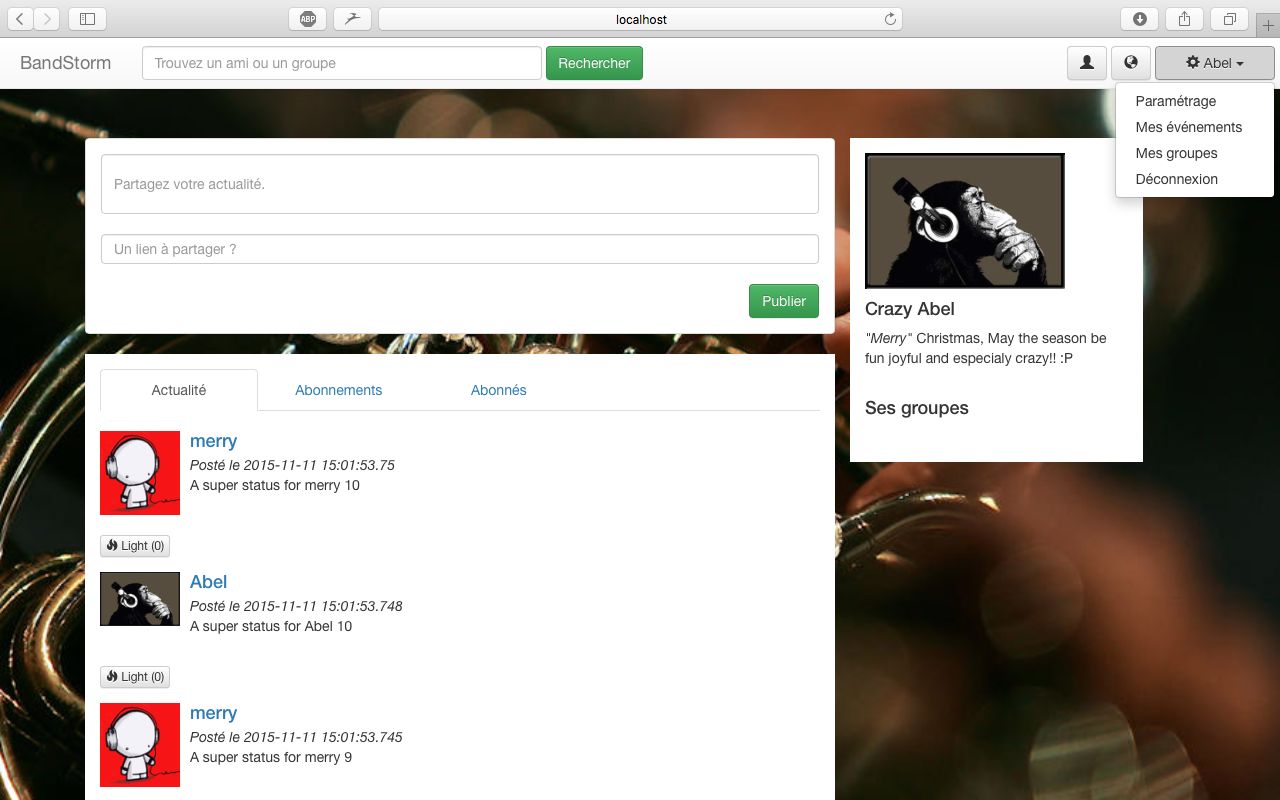
\includegraphics[width=0.95\linewidth]{images/Results/product/scshot4}
\caption{Page d'accueil des membres}
\label{fig:scshot4}
\end{figure}
}
\only<4>{
\begin{figure}
\centering
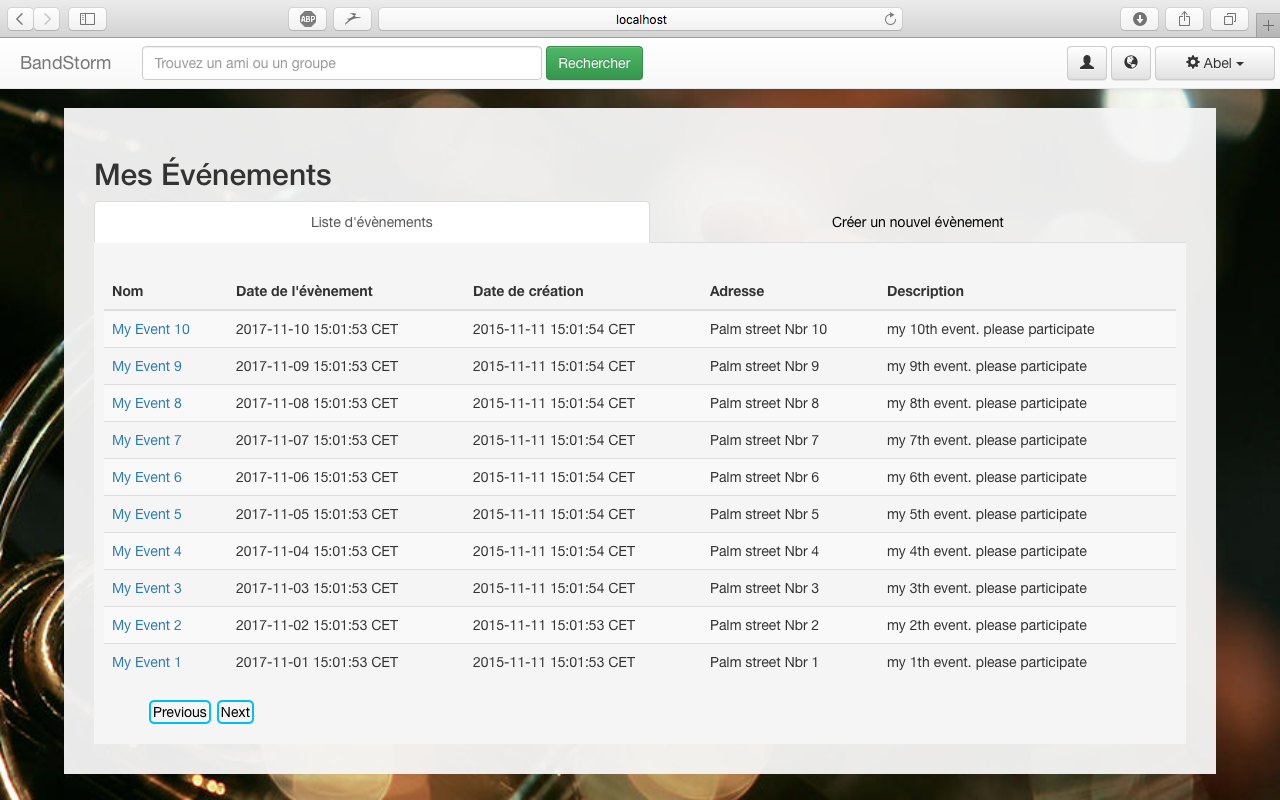
\includegraphics[width=0.95\linewidth]{images/Results/product/scshot5}
\caption{Liste des événements}
\label{fig:scshot5}
\end{figure}
}
\only<5>{
\begin{figure}
\centering
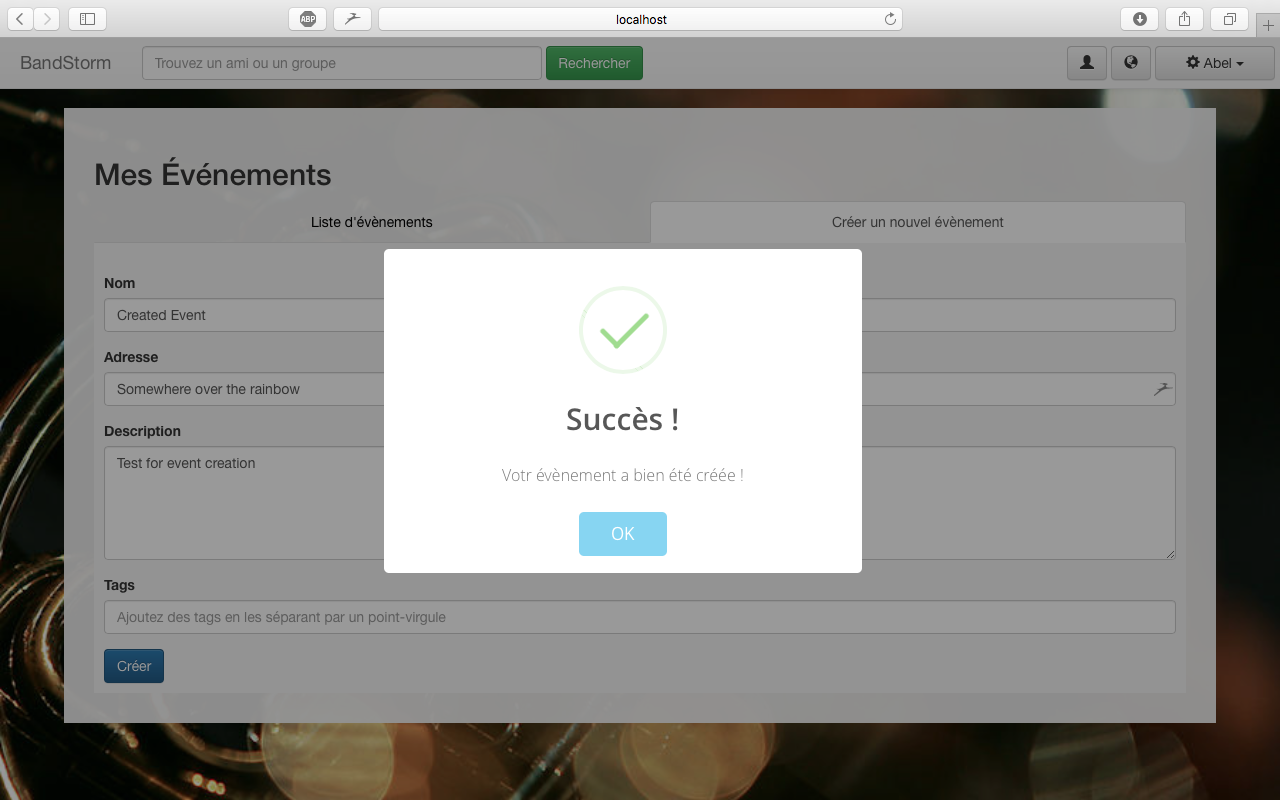
\includegraphics[width=0.95\linewidth]{images/Results/product/scshot6}
\caption{Création d'un événement}
\label{fig:scshot6}
\end{figure}
}
\only<6>{
\begin{figure}
\centering
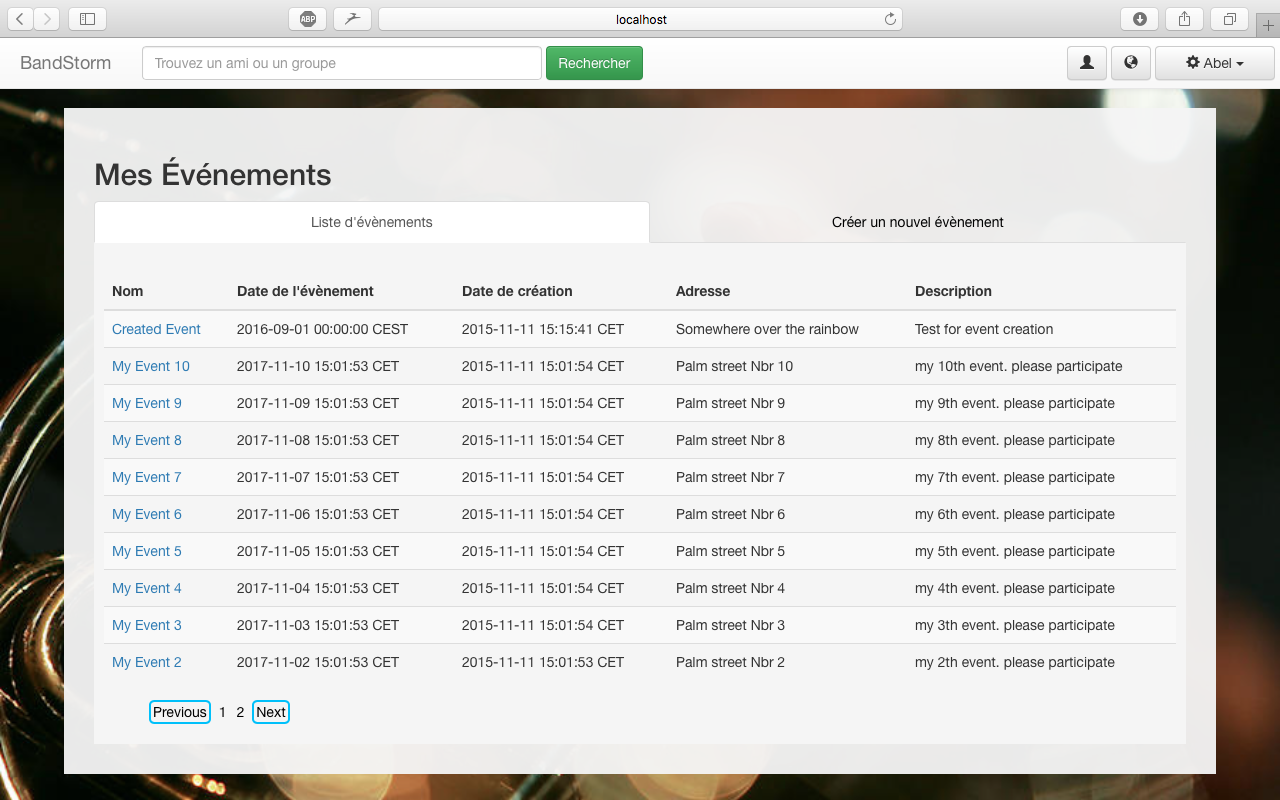
\includegraphics[width=0.95\linewidth]{images/Results/product/scshot7}
\caption{L'événement a été créé}
\label{fig:scshot7}
\end{figure}
}
\only<7>{
\begin{figure}
\centering
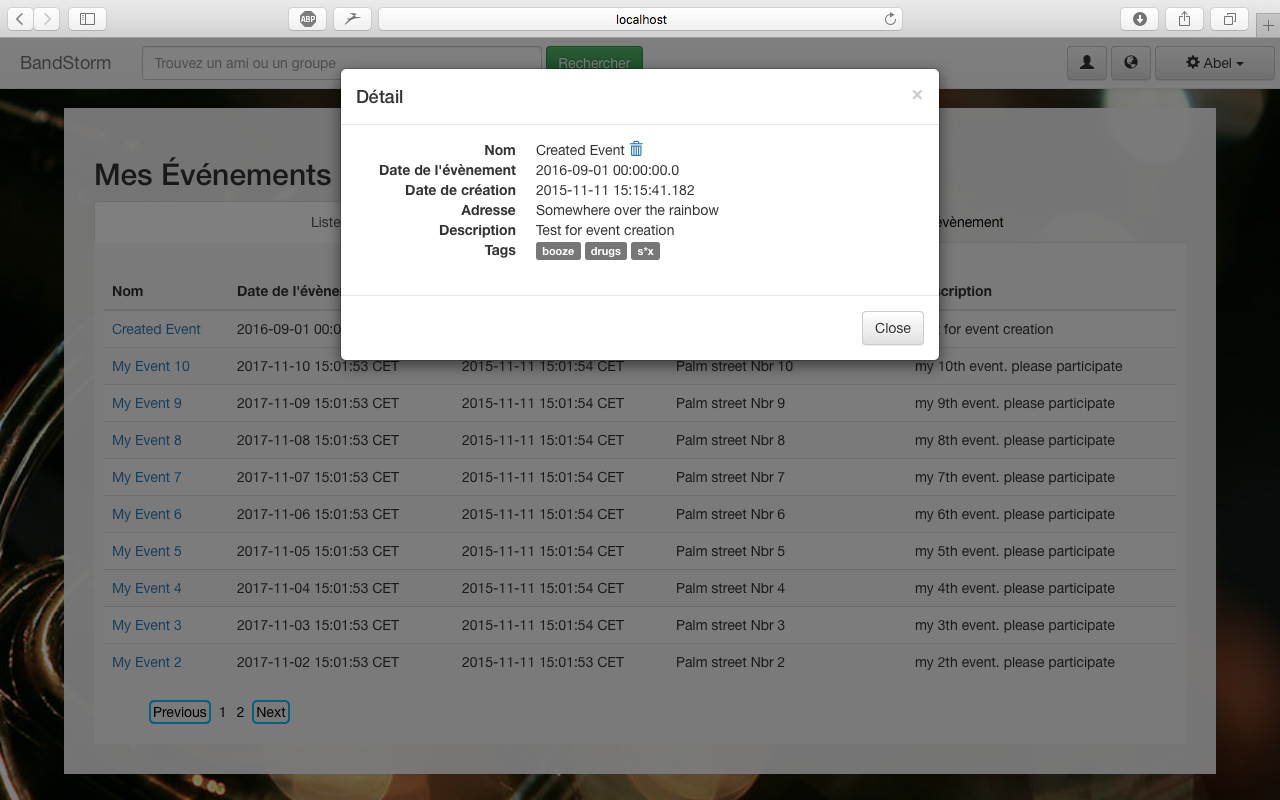
\includegraphics[width=0.95\linewidth]{images/Results/product/scshot8}
\caption{Détails de l'événement}
\label{fig:scshot8}
\end{figure}
}
\end{frame}

